\section{Results} % How well does the proposed solution perform?

% Compare the proposed solution against baseline and other solutions
%% Performance
%% Power
%% Area
%% Etc.
% Discuss the results
%% When and why does the proposed solution work well
%% When and why does the proposed solution work less well
\subsection{Sequential Prefetcher}
The sequential prefetcher was tested with a variety of prefetch
degrees and prefetch distances. Out of all the tests, ammp performed
significantly worse on all configurations. As we see later on, ammp
performes very well with RPT-LA, which indicates that ammp has a strided
access pattern. The results of the different variations are shown in
Figure~\ref{graph:seq}.
\begin{figure}[h]
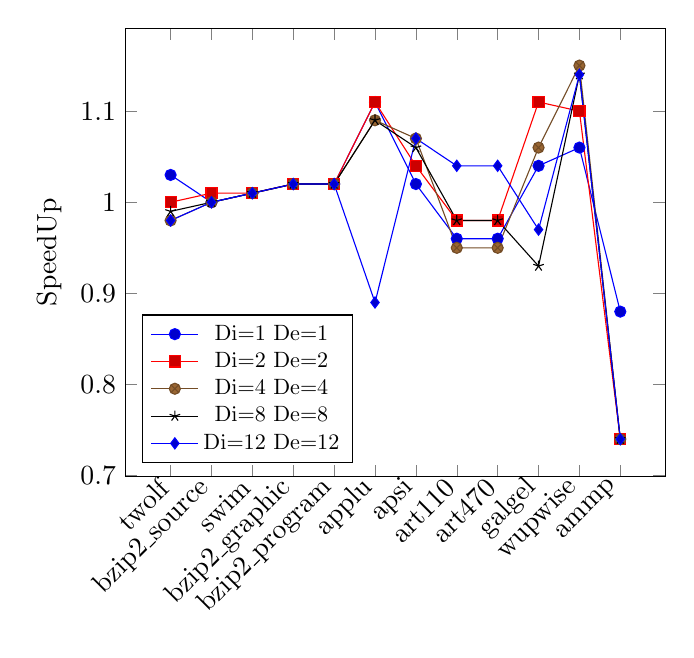
\begin{tikzpicture}
\begin{axis}[
    symbolic x
    coords={twolf,bzip2\_source,swim,bzip2\_graphic,bzip2\_program,applu,apsi,art110,art470,galgel,wupwise,ammp},
    xtick=data,
    x tick label style = {rotate=45,anchor=east},
    ylabel=SpeedUp,
    legend pos=south west,
    legend style = {nodes={scale=0.8, transform shape}}]
\addplot coordinates {
    (twolf,1.03)
    (bzip2\_source,1.00)
    (swim,1.01)
    (bzip2\_graphic,1.02)
    (bzip2\_program,1.02)
    (applu,1.11)
    (apsi,1.02)
    (art110,0.96)
    (art470,0.96)
    (galgel,1.04)
    (wupwise,1.06)
    (ammp,0.88)
};
\addplot coordinates {
    (twolf,1.00)
    (bzip2\_source,1.01)
    (swim,1.01)
    (bzip2\_graphic,1.02)
    (bzip2\_program,1.02)
    (applu,1.11)
    (apsi,1.04)
    (art110,0.98)
    (art470,0.98)
    (galgel,1.11)
    (wupwise,1.10)
    (ammp,0.74)
};
    \addplot coordinates {
    (twolf,0.98)
    (bzip2\_source,1.00)
    (swim,1.01)
    (bzip2\_graphic,1.02)
    (bzip2\_program,1.02)
    (applu,1.09)
    (apsi,1.07)
    (art110,0.95)
    (art470,0.95)
    (galgel,1.06)
    (wupwise,1.15)
    (ammp,0.74)
};
    \addplot coordinates {
    (twolf,0.99)
    (bzip2\_source,1.00)
    (swim,1.01)
    (bzip2\_graphic,1.02)
    (bzip2\_program,1.02)
    (applu,1.09)
    (apsi,1.06)
    (art110,0.98)
    (art470,0.98)
    (galgel,0.93)
    (wupwise,1.14)
    (ammp,0.74)
};
    \addplot coordinates {
    (twolf,0.98)
    (bzip2\_source,1.00)
    (swim,1.01)
    (bzip2\_graphic,1.02)
    (bzip2\_program,1.02)
    (applu,0.89)
    (apsi,1.07)
    (art110,1.04)
    (art470,1.04)
    (galgel,0.97)
    (wupwise,1.14)
    (ammp,0.74)
};
\legend{Di=1 De=1,Di=2 De=2,Di=4 De=4,Di=8 De=8,Di=12 De=12}
\end{axis}
\end{tikzpicture}
    \caption{Testing a sequential prefetcher with prefetch distance
      and degree set to 1, 2, 4, 8 and 12.}
\label{graph:seq}
\end{figure}
\subsection{Overall Performance}
The overall speedup of the five prefetchers is shown in
Figure~\ref{graph:base}. As expected, the more complex prefetchers
achieve a greater speedup.
\begin{figure}[h]
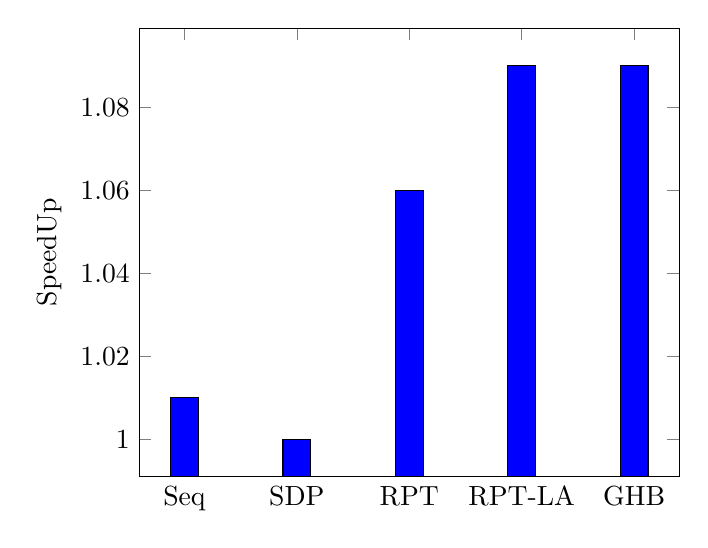
\begin{tikzpicture}
\begin{axis}[
    symbolic x coords={Seq,SDP,RPT,RPT-LA,GHB},
    xtick=data,
    ylabel=SpeedUp
    ]
\addplot[ybar,fill=blue] coordinates {
    (Seq,1.01)
    (SDP,1.00)
    (RPT,1.06)
    (RPT-LA,1.09)
    (GHB,1.09)
};
\end{axis}
\end{tikzpicture}
    \caption{Speedup of our implemented prefetchers compared to baseline.}
    \label{graph:base}
\end{figure}

\subsection{Test Specific Analysis}
The different prefetchers were tested using the SPEC CPU2000 benchmark
suite. From Figure~\ref{graph:tests} it is clear that SDP does not
succeed in creating any speedup. On the other hand, GHB and RPT-LA
show speedups in most of the tests.  They are very similar even though
the implementation is quite different.

\subsection{Table Sizes}
GHB and RPT-LA were tested with different table sizes, to find an
optimal configuration which minimizes size while maintaining
speedup. The effect of different table sizes on speedup is shown in
Figure~\ref{graph:tablesizes}. The effect on accuracy and coverage are
shown in Figure~\ref{graph:covaccghb} and
Figure~\ref{graph:covaccrpt}.

\begin{figure}[h]
\begin{tikzpicture}
\begin{axis}[
    symbolic x
    coords={twolf,bzip2\_source,swim,bzip2\_graphic,bzip2\_program,applu,apsi,art110,art470,galgel,wupwise,ammp,blank},
    xtick=data,
    ybar interval=0.7,
    x tick label style = {rotate=45,anchor=east},
    ylabel=SpeedUp,
    legend pos=north west
    ]
\addplot[fill=green] coordinates {
    (twolf,1.03)
    (bzip2\_source,1.00)
    (swim,1.01)
    (bzip2\_graphic,1.02)
    (bzip2\_program,1.02)
    (applu,1.11)
    (apsi,1.02)
    (art110,0.96)
    (art470,0.96)
    (galgel,1.04)
    (wupwise,1.06)
    (ammp,0.88)
    (blank,1)
};
\addplot[fill=gray] coordinates {
    (twolf,1.00)
    (bzip2\_source,1.00)
    (swim,1.00)
    (bzip2\_graphic,1.00)
    (bzip2\_program,1.00)
    (applu,0.99)
    (apsi,1.00)
    (art110,1.00)
    (art470,1.00)
    (galgel,1.00)
    (wupwise,1.00)
    (ammp,1.00)
    (blank,1)
};
    \addplot[fill=black] coordinates {
    (twolf,0.99)
    (bzip2\_source,1.00)
    (swim,1.01)
    (bzip2\_graphic,1.01)
    (bzip2\_program,1.04)
    (applu,1.05)
    (apsi,1.07)
    (art110,1.06)
    (art470,1.06)
    (galgel,1.09)
    (wupwise,1.25)
    (ammp,1.63)
    (blank,1)
};
    \addplot[black, fill=yellow] coordinates {
    (twolf,0.99)
    (bzip2\_source,1.00)
    (swim,1.01)
    (bzip2\_graphic,1.02)
    (bzip2\_program,1.04)
    (applu,1.05)
    (apsi,1.06)
    (art110,1.06)
    (art470,1.06)
    (galgel,1.11)
    (wupwise,1.25)
    (ammp,1.66)
    (blank,1)
};
\legend{Seq,SDP,GHB,RTP-LA}
\end{axis}
\end{tikzpicture}
    \caption{Results for the tests in the SPEC CPU2000 benchmark suite.}
    \label{graph:tests}
\end{figure}


\begin{figure}
  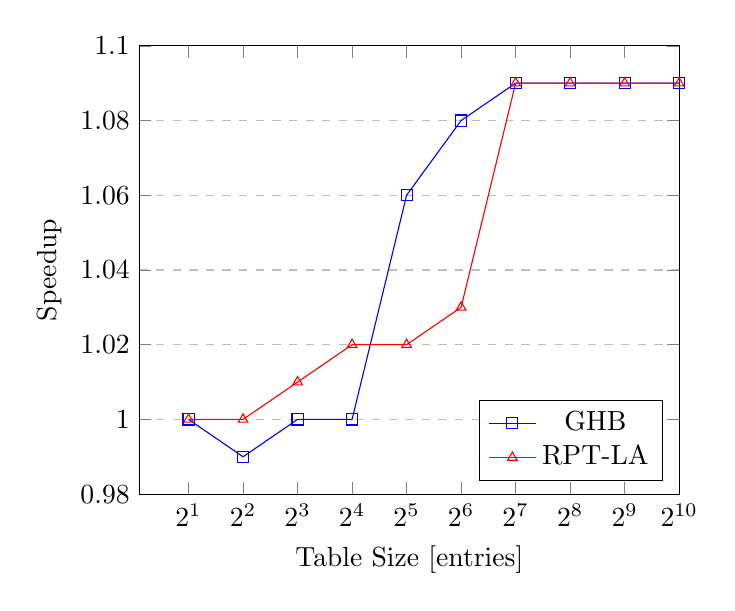
\begin{tikzpicture}
    \begin{axis}[
    % width = \columnwidth,
    xlabel={Table Size [entries]},
    ylabel={Speedup},
    xmode=log,
    log basis x={2},
    xmin=0, xmax=1024,
    ymin=0.98, ymax=1.1,
    xtick={2,4,8,16,32,64,128,256,512, 1024},
    ymajorgrids=true,
    grid style=dashed,
    legend pos = south east
    ]
    \addplot[
    color=blue,
    mark=square,
    ]
    coordinates {
      (2,1)(4,0.99)(8,1)(16,1)(32,1.06)(64,1.08)(128,1.09)(256,1.09)(512,1.09)(1024,1.09)
    };
    \addplot[
    color=red,
    mark=triangle,
    ]
    coordinates {
      (2,1)(4,1)(8,1.01)(16,1.02)(32,1.02)(64,1.03)(128,1.09)(256,1.09)(512,1.09)(1024,
      1.09)
    };
    \legend{GHB, RPT-LA}
    \end{axis}
  \end{tikzpicture}
  \caption{Speedup for varying table sizes in RPT-LA and GHB}
  \label{graph:tablesizes}
\end{figure}

\begin{figure}
  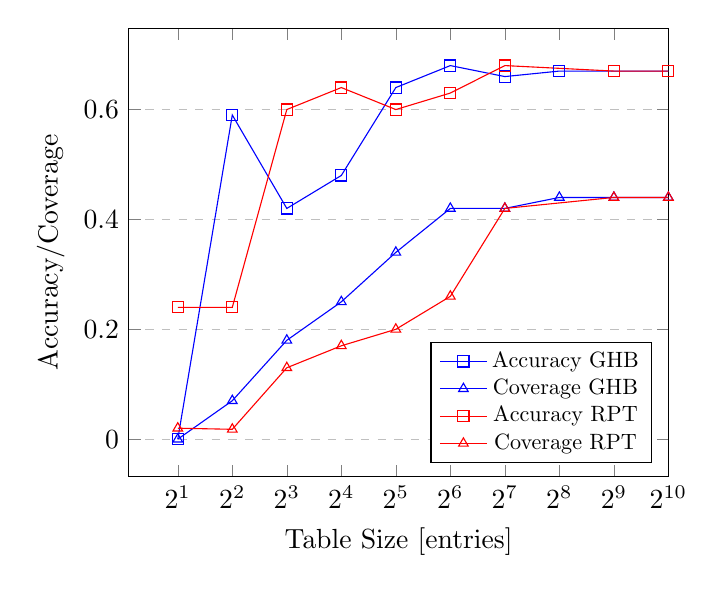
\begin{tikzpicture}
    \begin{axis}[
      xlabel={Table Size [entries]},
      ylabel=Accuracy/Coverage,
      xmode=log,
      log basis x={2},
      xmin=0, xmax = 1024,
      xtick={2,4,8,16,32,64,128,256,512, 1024},
      legend pos = south east,
      grid style=dashed,
      ymajorgrids=true,
      legend style = {nodes={scale=0.8, transform shape}},
      ]
      \addplot[color = blue, mark = square]
      coordinates {
        (2,0)(4,0.59)(8,0.42)(16,0.48)(32,0.64)(64,0.68)(128,
        0.66)(256, 0.67)(512, 0.67)(1024,0.67)
      };
      \addplot[color = blue, mark = triangle]
      coordinates {
        (2,0)(4,0.07)(8,0.18)(16,0.25)(32,0.34)(64,0.42)(128,0.42)(256,0.44)(512,0.44)(1024,0.44)
      };
      \addplot[color = red, mark = square]
      coordinates {
        (2,0.24)(4,0.24)(8,0.6)(16,0.64)(32,0.60)(64,0.63)(128,
        0.68)(512, 0.67)(1024,0.67)
      };
      \addplot[color = red, mark = triangle]
      coordinates {
        (2,0.02)(4,0.018)(8,0.13)(16,0.17)(32,0.2)(64,0.26)(128,
        0.42)(512, 0.44)(1024,0.44)
      };
      \legend{Accuracy GHB, Coverage GHB, Accuracy RPT, Coverage RPT}
    \end{axis}
  \end{tikzpicture}
  \caption{Accuracy And Coverage for varying table sizes in GHB and RPT-LA}
  \label{graph:covaccghb}
\end{figure}

\subsection{Size}
As seen in Figure~\ref{graph:tablesizes} and~\ref{graph:covaccghb},
the optimal table size for GHB and RPT-LA is $2^7=128$ entries. The
GHB implementation uses an index table of size 90 entries. Therefore,
the approximate memory usage of GHB is (128 entries * 16 bytes/entry)
+ (90 entries * 16 bytes/entry) = 3488 bytes. The approximate memory
usage of RPT-LA is 128 entries * 16 bytes/entry = 2048 bytes.
